\section{The problem}
Apply the general method to the new target matrix
\begin{equation}
  \A{} = \mat{ccc}
  {
  0 & 3 & 0 \\
  1 & 2 & 2
  }
\end{equation}
and follow the steps in table \eqref{tab:3:input} to produce an SVD.\\

Diagnosis: the target matrix has rank 2 due to two independent rows. Therefore we can define the shapes of the component matrices as show in figure \eqref{fig:232}.
\begin{equation}
  \A{}\in\real{\by{2}{3}}_{2}.
\end{equation}
\begin{figure}[htbp] %  figure placement: here, top, bottom, or page
   \centering
%   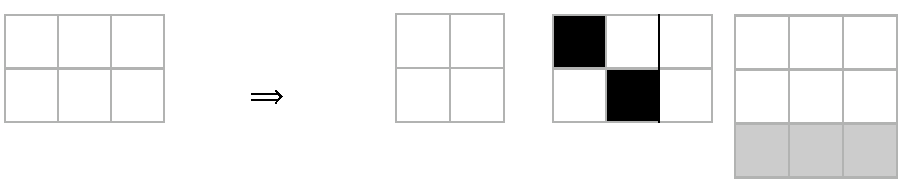
\includegraphics[ ]{pdf/general/svd_02_03_02} 
   \includegraphics[ ]{pdf/general/C232} 
   \caption[Shapes and dimensions]{The shapes and dimensions for the pending decomposition are determined by the shape of the target matrix. The rank tells us how many singular values we will find.}
   \label{fig:232}
\end{figure}
%%%

%%
\subsection{Compute the adjoint matrix $\A{T}$}
\begin{equation}
  \A{} = \mat{cc}
  {
  0 & 1 \\
  3 & 2 \\
  0 & 2
  }.
\end{equation}

%%
\subsection{Compute the product matrix $\W{x}$}
\begin{equation}
  \W{x}=\A{T}\A{}= \mat{ccc}{
 1 &  2 & 2 \\
 2 & 13 & 4 \\
 2 &  4 & 4}
\label{eq:problemgen:Wx}
\end{equation}

%%
\subsection{Find the eigenvalues of $\W{x}$}
We could solve this system for eigenvectors and eigenvalues. But the product matrix $\W{y}$ is a smaller and simpler system to resolve. So to reduce the amount of labor we will work with the other product matrix
\begin{equation}
  \W{y}=\A{}\,\A{T} =
\left[
\begin{array}{cc}
 9 & 6 \\
 6 & 9
\end{array}
\right].
\label{eq:problemgen:Wy}
\end{equation}
Details are in the appendix allowing a freedom to touch upon just the high notes. 

Start with a some simplification: remove common factors from the product matrix. To wit
\begin{equation}
  \W{y}=3\W{y}'.
  \label{eq:scale}
\end{equation}

To find the eigenvalues, find the the roots of the \index{characteristic polynomial} characteristic polynomial defined by
\begin{equation}
  p(\lambda) = \det \paren{\W{y}'-\lambda \I{2}} =
  \det \mat{cc}
  {
  3-\lambda & 2 \\
  2 & 3-\lambda
  }.
\end{equation}

In this instance we find
\begin{equation}
  p(\lambda) = \lambda^{2} - 6\lambda + 5
\end{equation}
which is easily factored. Extracting the roots to $p(\lambda) = 0$ yields $\lambda = \lst{5,1}$. Accounting for the scale factor in \eqref{eq:scale} we say the eigenvalue spectrum for the product matrix $\W{y}$ is given by
\begin{equation}
  \lambda = \lst{15, 3}
\end{equation}

\textbf{Caution:} Always arrange the eigenvalues in \textit{decreasing} magnitude.

%%
\subsection{Compute the singular values $\sigma_{k}$}
The singular values are the square root of the non-zero eigenvalues of the product matrices:
\begin{equation}
  \sigma = \sqrt{\lambda} = \lst{\sqrt{15},\sqrt{3}}.
\end{equation}

%%
\subsection{Build the $\sig{}$ matrix}
The $\sig{}$ matrix of singular values has the same dimensions are the target matrix. Populate the upper diagonal with singular values:
\begin{equation}
  \A{} = \mat{cc|c}
  {
  \sqrt{15} & 0 & 0 \\
  0 & \sqrt{3}  & 0
  }
\end{equation}

%%
\subsection{Find the eigenvectors of the product matrix $\W{x}$}
The eigenvalue problem for this example is this
\begin{equation}
  \W{x}\lambda_{k} = \lambda_{k} x_{k}, \quad k=\lst{1,\rho}.
  \label{eq:raw:ev}
\end{equation}
Here $x_{k}$ is the eigenvector of interest. Notice that we skip any cases where $\lambda=0$. Yes, this would provide null vectors, but they would not be an orthogonal set.

The canonical method for solving equation \eqref{eq:raw:ev} is to express it as a null space problem as they are easier to solve:
\begin{equation}
  \paren{\W{x} - \lambda_{k}\I{3}} = \zero, \quad k=\lst{1,\rho}.
\end{equation}
The two cases follow. Both will be solved by augmented reduction or EAR.
\begin{enumerate}
\item For $k=1$. The source matrix is given by
\begin{equation}
\W{x}-15\I{3} =
\left[
\begin{array}{rrr}
 -14 & 2 & 2 \\
 2 & -2 & 4 \\
 2 & 4 & -11
\end{array}
\right]. 
\end{equation}
The augmented system has this final form
\begin{multline}
\frac{1}{12}
\left[
\begin{array}{rrr}
 5  & 29 & 12 \\
 -1 & -7 & 0 \\
 6  & 30 & 12
\end{array}
\right]
\mat{rrr|ccc}
{
-14 & 2 & 2 & 1 & 0 & 0 \\
 2 & -2 & 4 & 0 & 1 & 0 \\
 2 & 4 &-11 & 0 & 0 & 1
}\\
=
\mat{crr|rrc}
{
1 & 0 & -\frac{1}{2}  &  \frac{5}{12} & \frac{29}{12} & 1 \\
0 & 1 & -\frac{5}{2}  & -\frac{1}{12} & -\frac{7}{12} & 0 \\[4pt]\hline\hline
0 & 0 & 0             &  \frac{1}{2}  & \frac{5}{2}   & 1
}.
\end{multline}
The double horizontal lines are drawn to accentuate the boundary of the null vectors. The row vectors of interest accompany the zero vectors on the bottom of the matrix on the right. In this case there is just one vector:
\begin{equation}
  x_{1}^{\mathrm{T}} = \mat{ccc}{1&5&2}
\end{equation}
After normalization, we have the first column in the domain matrix:
\begin{equation}
  \X{}_{*,1} = \hat{x}_{1} = \frac{1}{\sqrt{30}}\mat{c}{1\\5\\2}.
\end{equation}
\item For $k=2$
\begin{equation}
\W{x}-3\I{3} =
\left[
\begin{array}{rrr}
 -2 & 2 & 2 \\
 2 & 10 & 4 \\
 2 & 4 & 1
\end{array}
\right].
\end{equation}
The augmented system has this final form
\begin{multline}
\frac{1}{12}
\left[
\begin{array}{crc}
 1 & -5 & 12 \\
 1 &  1 & 0 \\
 6 & -6 & 12
\end{array}
\right]
\mat{rrr|ccc}
{
-2 & 2  & 2 & 1 & 0 & 0 \\
 2 & 10 & 4 & 0 & 1 & 0 \\
 2 & 4  & 1 & 0 & 0 & 1
}\\
=
\mat{ccr|crc}
{
1 & 0 & -\frac{1}{2}  &  \frac{1}{12} & -\frac{5}{12} & 1 \\
0 & 1 &  \frac{1}{2}  &  \frac{1}{12} &  \frac{1}{12} & 0 \\[4pt]\hline\hline
0 & 0 & 0             &  \frac{1}{2}  & -\frac{1}{2}  & 1
}.
\end{multline}
\end{enumerate}
With normalization, we have the second column in the domain matrix:
\begin{equation}
  \X{}_{*,2} = \hat{x}_{2} = \frac{1}{\sqrt{6}}\mat{r}{1\\-1\\2}.
\end{equation}

%%
\subsection{Construct a null space for the domain}
Part of the confusion about the decomposition comes from the wonderful fact that there are some permutations in the path and multiple ways to approach some steps.

Here there are different ways to construct this third vector and assure that it is perpendicular to the first two vectors. We choose to use the cross-product.

The cross-product between two \vvv s is computed as this
\begin{equation}
\mat{c}{x_{1}\\x_{2}\\x_{3}}
\times
\mat{c}{y_{1}\\y_{2}\\y_{3}}
=
\det
\mat{ccc}
{
\hat{i} & \hat{j} & \hat{k} \\
  x_{1} & x_{2}   & x_{3}   \\
  y_{1} & y_{2}   & y_{3}   \\
}
=
\mat{c}
{
x_{2}y_{3}-x_{3}y_{2} \\
x_{3}y_{1}-x_{1}y_{3} \\
x_{1}y_{2}-x_{2}y_{1} 
}.
\end{equation}
The solitary null space vector is
\begin{equation}
u_{1} = x_{1} \times x_{2} =
\mat{c}{1\\5\\2}
\times
\mat{r}{1\\-1\\2}
=
\mat{r}
{
 2 \\
 0 \\
-1 
}.
\end{equation}
Therefore
\begin{equation}
  \X{}_{*,3} =\hat{u}_{1} = \frac{1}{\sqrt{5}}
\mat{r}
{
 2 \\
 0 \\
-1 
}.
\end{equation}

%%
\subsection{Assemble the domain matrix $\X{}$}
The normalization busies the appearance:
\begin{equation}
  \X{} = 
\left[
\begin{array}{ cr >{\columncolor{ltgray}}r }
  \frac{1}{\sqrt{30}} & \frac{ 1}{\sqrt{6}} & \frac{-2}{\sqrt{5}}\\
  \frac{5}{\sqrt{30}} & \frac{-1}{\sqrt{6}} & 0 \\
  \frac{2}{\sqrt{30}} & \frac{ 2}{\sqrt{6}} & \frac{ 1}{\sqrt{5}}\\
\end{array}
\right].
\end{equation}

A useful alternative presentation of this matrix is to write it as column vectors as shown here:
\begin{equation}
\X{}=
  \mat{c|c|>{\columncolor{ltgray}}c}
  {
  \frac{1}{\sqrt{30}} \mat{r}{1\\5\\2} &
  \frac{1}{\sqrt{6}}  \mat{r}{1\\-1\\2} &
  \frac{1}{\sqrt{5}}  \mat{r}{2\\0\\1}
  }.
\end{equation}
This defeats the camouflage of the normalization constants and reminds us of the significance of the columns. It also simplifies the visual check of orthogonality.

%%
\subsection{Solve for $y_{k}$}
A vital formula needed for \index{jumping between domains}jumping between domain and codomain is this
\begin{equation}
  \A{}\X{}_{*,k} = \sigma_{k} \Y{}_{*,k}, \quad k=\lst{1,\rho}.
  \label{eq:vital}
\end{equation}
\begin{enumerate}
\item For $k=1$
For the first normalized vector in the codomain we need to solve
\begin{equation}
  \begin{split}
    \A{}\X{}_{*,1} &= \sigma_{1} \Y{}_{*,1}, \\
    \mat{ccc}
    {0 & 3 & 0\\
     1 & 2 & 2
    }
    \frac{1}{\sqrt{30}}
    \mat{c}{1\\5\\2}
    & = 
    \sqrt{15} \Y{}_{*,1}.
  \end{split}
\end{equation}
The solution is
\begin{equation}
  \Y{}_{*,1} = \frac{1}{\sqrt{2}}\mat{c}{1\\1}.
\end{equation}
\item For $k=2$
It may be tempting to guess the second and final vector in the codomain matrix; there are only two possible choices. But to do so would entail the risk of placing the minus sign in the wrong place. So much of the decomposition keeps the arbitrary signs in consistent use. After working out the details, the solution to
\begin{equation}
  \A{}\X{}_{*,2} = \sigma_{2} \Y{}_{*,2}
\end{equation}
is the vector
\begin{equation}
  \Y{}_{*,2} = \frac{1}{\sqrt{2}}\mat{r}{-1\\1}
\end{equation}
\end{enumerate}

%%
\subsection{Construct a null space for the codomain}
There is no null space for the codomain; the target matrix has full row rank.

%%
\subsection{Assemble the codomain matrix $\Y{}$}
The codomain matrix is given by
\begin{equation}
  \Y{} = \frac{1}{\sqrt{2}}
  \mat{rr}{1 & -1\\1 & 1}.
\end{equation}

%%
\subsection{Assemble and verify the decomposition}
The formal decomposition is
\begin{equation}
  \boxed{
  \begin{array}{ccccc}
    \A{} &=& \Y{} & \sig{} & \X{T}\\
  \mat{ccc}
  {
  0 & 3 & 0 \\
  1 & 2 & 2
  } 
  &=&
  \frac{1}{\sqrt{2}}
  \mat{rr}{1 & -1\\1 & 1}
  &
  \mat{cc|c}
  {
  \sqrt{15} & 0 & 0 \\
  0 & \sqrt{3}  & 0
  }
  &
  \mat{ crr }
 {\frac{1}{\sqrt{30}} & \frac{5}{\sqrt{30}} & \frac{2}{\sqrt{30}}\\
  \frac{ 1}{\sqrt{6}} & \frac{-1}{\sqrt{6}} & \frac{2}{\sqrt{6}} \\
  \rowcolor{ltgray}
  \frac{-2}{\sqrt{5}} & 0 & \frac{1}{\sqrt{5}}}\\[25pt]
  \end{array}.
  }
  \label{eq:general:ysxt}
\end{equation}

The best way to insure that all the signs on the entries in the domain matrices are correct is to verify the decomposition:
\begin{equation}
  \begin{split}
    \A{} &= \Y{}\paren{\sig{}\,\X{T}},\\
     &=
  \stwo
  \mat{rr}{1 & -1\\1 & 1}
  \paren{
  \stwo
  \mat{crc}
  {
  1 & 5  & 2 \\
  1 & -1 & 2
  }}, \\
  &=
  \mat{ccc}
  {
  0 & 3 & 0 \\
  1 & 2 & 2
  }.
  \end{split}
  \label{eq:gen:soln}
\end{equation}

\endinput